% =====================================================================
% main.tex -- StellarOrion Progress Report, Week 17
%
% SKELETON BUILD. The frame STRUCTURE, sectioning, navigation and
% house-style typography are final. Body content is left as marked
% placeholders for the content thread (GoalThread6).
%
% =====================================================================
% PRESENTATION TEXT BUDGET -- READ BEFORE ADDING ANY WORDS
% ---------------------------------------------------------------------
% This is a SLIDE DECK, not a document. The governing rule, enforced by
% \MaxTextLines below:
%
%   * MAXIMUM 1-2 LINES of text per frame. Hard cap, not a guideline.
%   * EACH FRAME IS DOMINATED BY AN IMAGE PLOT. The plot is the content.
%     Text is the caption, never the payload.
%   * NO BULLET LISTS. A bullet list on a slide is a paragraph that
%     happens to be indented, which is the failure this budget exists to
%     prevent. If a frame needs more than two lines, it needs to be split
%     into two frames, not given a third bullet.
%   * NO EM-DASHES (U+2014 / `---`). The thesis completed a measured
%     em-dash removal with zero residual; slide prose keeps that rule.
%   * EVERY NUMBER MUST CITE ITS SOURCE FILE. Nothing ships unsourced.
%
% These are not preferences inherited from a style guide. They are the
% reasons the existing PowerPoint decks could not be converted: the Week 14
% deck carries 63 words total, 0 speaker notes, and its content is 2
% embedded mp4 plus 9 rasters. There is no text there to port, so this deck
% is authored from verified repository state and must be built to the
% budget above rather than padded to fill frames.
%
% HOW TO PLACE AN IMAGE PLOT
%   \PlotFrame{<frametitle>}{<caption, 1-2 lines max>}{<image file>}
% The macro in preamble.tex reserves the frame's vertical space for the
% plot and draws the caption beneath it, so a plot is never squeezed by
% the text above it. Use it rather than hand-rolling figure blocks.
%
% Citation: Beamer -- https://ctan.org/pkg/beamer
%           pdfTeX 3.141592653-2.6-1.40.29 (TeX Live 2026)
% =====================================================================
% NARRATION REVAMP -- TARGET STRUCTURE (PLACEHOLDER SCAFFOLD ONLY)
% ---------------------------------------------------------------------
% Owner directive, 2026-10-21: "for the latest one, create placeholder
% for these. don't do anything or fill in anything yet", followed by
% "This is the structure that we need to have on the latest latex one"
% and "add it into the comments too for this structure too".
%
% WHAT THIS BLOCK IS
%   It records the narration order the deck must end up in. Nothing in
%   it is filled in. Every item below has exactly one placeholder frame
%   in the final section "NARRATION REVAMP: PLACEHOLDER SCAFFOLD" at
%   the end of this file, and each placeholder frame carries, in its
%   own comment, the position that frame must occupy once its real
%   content exists.
%
% THE STRUCTURE AS GIVEN BY THE OWNER
%
%   [ Intro start ]
%     0. title start
%   [ intro end ]
%
%   [ recall start ]
%     1. Latar belakang overview
%     2. Tujuan objective? (all and 2-3 points), Research Scope limit
%     3. Methodology (update or not?) (Graphical Framework flowchart)
%        (and it's (each steps and methodology) definition)
%        (Detailed methodology)
%        (The reasoning too)
%     4. Previous issues
%   [ recall end ]
%
%   [ Current progress start ]
%     5. Overall Progress on the research?
%        (Not the technical detail on the Resolution)
%   [ Current progress end ]
%
%     6. The progress issue and the resolution (the attempt) and the
%        update (let's say DSMC, Narration)
%
%   [ Ending start ]
%     Conclusion (How close to the objective and does it answers the
%     previous issue?)
%   [ Ending end ]
%
%   CFD (What's required?) and Optimized (What's required?) plot:
%   (Lebih di tulisan), Reference find paper then show on the next or
%   point 6
%
% TRANSLITERATION NOTE (house rule, not an edit of the owner's wording)
%   The owner's block marks its boundaries with U+2014 em-dashes. This
%   deck carries a measured zero-em-dash rule (see the PRESENTATION TEXT
%   BUDGET block above), so those boundary marks are written here as
%   [ ... ] brackets with ASCII hyphens. The wording of the structure
%   itself is the owner's, unaltered.
% =====================================================================
\documentclass[aspectratio=169,11pt]{beamer}

% =====================================================================
% preamble.tex -- house style for the Week 17 progress deck
%
% Every setting here is inherited from the ITB thesis, not invented.
% Source: Lost+Found/ProgressReport/CurrentThesisFinalReport/preamble.tex
% Contract documented in GoalThread5.md -> "House style contract".
% =====================================================================

% ---------------------------------------------------------------------
% TYPOGRAPHY
% The thesis sets T1 encoding + mathptmx (Times-family) + dsfont
% (preamble.tex lines 112, 113, 117). Beamer defaults to Computer Modern
% Sans, which would make the deck look like a different institution's
% document, so the Times stack is restored here. T1 comes first because
% fontenc must be loaded before any font selection takes effect.
%
% Citation: mathptmx -- https://ctan.org/pkg/pxfonts
%           dsfont   -- https://ctan.org/pkg/dstds
% ---------------------------------------------------------------------
\usepackage[T1]{fontenc}
\usepackage{mathptmx}
\usepackage{dsfont}

\usepackage{booktabs}   % thesis uses it for tabular rules; tables are expected
\usepackage{microtype}  % kpsewhich-confirmed present in this TeX Live install

% tikz provides the page-anchored overlay used by \ITBTitleBackground to paint
% the turquoise title band. It MUST be loaded explicitly.
%
% MEASURED, after getting this wrong first: beamer loads pgf but does NOT
% load the tikz front end. With no \usepackage{tikz} the build reports
% "LaTeX Error: Environment tikzpicture undefined" at main.tex:73, followed
% by a cascade ("Missing number, treated as zero", and
% "\begin{beamer@framepauses} ... ended by \end{tikzpicture}").
% Being able to RESOLVE tikz.sty with kpsewhich proves the file is installed,
% not that it is loaded -- availability and loading are different facts.
% Citation: tikz -- https://ctan.org/pkg/pgf
\usepackage{tikz}
\usetikzlibrary{calc,shadings}

% accsupp is REQUIRED, not decorative: the ITB emblem is an image that adds
% no information a screen reader needs (the institution is already named in
% the text on the same frame), and an unlabelled image is announced as an
% unnamed graphic, failing WCAG 1.1.1. The thesis marks it decorative on the
% cover via \BeginAccSupp/\EndAccSupp, and this deck repeats that treatment.
% Note accsupp exposes only the COMMAND form, never a begin/end environment.
% Citation: accsupp -- https://ctan.org/pkg/accsupp
\usepackage{accsupp}

% =====================================================================
% PALETTE -- TURQUOISE + GHIBLI, FLAT
%
% REVISION HISTORY (read this before "correcting" the palette back).
% v1  pure monochrome. This is what the ITB thesis measures as:
%     `grep -c definecolor preamble.tex` returns 0, and a repo-wide scan of
%     all 18 thesis .tex files for \definecolor or \color{ returns nothing.
%     That contract is recorded in GoalThread5.md and is NOT deleted from it.
% v2  pastel + turquoise (saturated teal), on the user's direction.
% v3  TURQUOISE + GHIBLI -- the current version, on the user's direction.
%     "Ghibli" here means the Miyazaki palette: DESATURATED and DUSTY rather
%     than vivid. Warm parchment grounds, sage-tinted accents, and a muted
%     teal that reads as weathered water rather than swimming-pool teal. v2's
%     #00695C was too clean and too saturated for that; v3 pulls the hue
%     toward grey-green and drops the chroma.
% The user is the authority on the look of their own progress deck, so the
% palette follows their direction. The measured monochrome finding remains
% true of the THESIS, which is a different document.
%
% WHY A GUST-OF-WIND CHECK MATTERS HERE: the v2 accents were chosen for
% contrast and read as clinical teal on a projector. Ghibli's palette is
% built on lower chroma, which is exactly the property that makes colours
% fail a contrast test. So every pair below is measured AFTER being picked
% for mood, and the mood colours that failed were darkened rather than used.
%
% THERE IS NO \usetheme{flat}. This was verified with kpsewhich, which is
% authoritative for the TeX tree:
%   beamerthemeflat.sty        MISSING
%   beamerouterthemeinfinity.sty MISSING
% The "flat" look people mean is the infinity outer theme plus a
% structure-only colour scheme, and neither is installed here either. So
% the flat aesthetic is BUILT BY HAND below: solid fills, thin rules, no
% gradients, no bevels, no shadows, no rounded 3-D chrome. Nothing here
% depends on a theme file that might be missing on another machine.
%
% Citation: beamer colour themes -- https://ctan.org/pkg/beamer
%           xcolor        -- https://ctan.org/pkg/xcolor
% =====================================================================

% xcolor is still loaded with `[table]`, exactly as the thesis loads it, so
% \cellcolor keeps working for any table added later. The palette below is
% the only reason colour appears in this deck.
\usepackage[table]{xcolor}

% ---------------------------------------------------------------------
% PALETTE DEFINITIONS
%
% AXIOM: every foreground/background pair actually used below was measured
% for WCAG contrast before being written down, not chosen by eye. The
% measured ratios are recorded next to each colour so a later edit cannot
% silently break legibility.
%
% THEORY: WCAG 2.1 contrast ratios are computed from relative luminance per
% https://www.w3.org/TR/WCAG21/#dfn-relative-luminance . Thresholds used:
% 4.5:1 for normal text, 3:1 for large/bold text, 3:1 for meaningful
% non-text graphics (WCAG 1.4.11).
%
% APPLICATION: content frametitles, body text, the frame counter, blocks and
% the title band.
%
% MEASURED RATIOS (computed by script, not eyeballed):
%   white #FFFFFF   on band #2F6B69 = 6.13:1  AA
%   parch #F2EADA   on band #2F6B69 = 5.12:1  AA  (subtitle, SMALL text)
%   sand  #EDE4CE   on band #2F6B69 = 5.21:1  AA  (author/date, SMALL text)
%   ITB emblem (white art) on band  = 6.13:1  AA
%   frametitle #2F4F4D on cream #F5EFE0 = 7.80:1  AAA
%   body ink   #33302B on white       = 13.14:1  AAA
%   body ink   #33302B on #E8EEE9     = 11.16:1  AAA
%   counter #2F4F4D on sage #CFDDD8   = 6.39:1  AA
%   accent #5E918C on cream (rule)    = 3.10:1  >=3.0 non-text OK
%
% MOOD-FIRST, THEN MEASURED -- and the failures are recorded so they are not
% re-introduced by eye. Ghibli's palette is BUILT on low chroma, which is
% exactly the property that fails a contrast test, so the pretty dusty teals
% were tried first and rejected on measurement:
%   #4A8A86 gives white only 3.98:1 (large-text only)
%   #7FA9A4 on cream = 2.26:1, #8FB5B0 on cream = 1.95:1 (both FAIL)
% Hence band #2F6B69 and accent #5E918C: the darkest tones that still read
% dusty rather than clinical. The CREAM grounds are safe BECAUSE they are
% light, and they are what carries the Ghibli warmth.
% ---------------------------------------------------------------------
\definecolor{SOGhibliBand}{HTML}{2F6B69}   % title band fill; white 6.13:1
\definecolor{SOGhibliInk}{HTML}{2F4F4D}   % frametitle / counter fg
\definecolor{SOGhibliAcc}{HTML}{5E918C}   % rules + accents; 3.10:1 on cream
\definecolor{SOGhibliDeep}{HTML}{243F3D}  % deepest teal, sparing use
\definecolor{SOGhibliCream}{HTML}{F5EFE0} % frametitle band (parchment)
\definecolor{SOGhibliSage}{HTML}{CFDDD8}  % counter band (pale sage)
\definecolor{SOGhibliMist}{HTML}{E8EEE9}  % block body (cool parchment)
\definecolor{SOGhibliSand}{HTML}{EDE4CE}  % block accent (warm)
\definecolor{SOGhibliParch}{HTML}{F2EADA}% subtitle/author on band
\definecolor{SOGhibliBody}{HTML}{33302B}  % body text; 13.14:1 on white

\setbeamercolor{structure}{fg=SOGhibliAcc}
\setbeamercolor{frametitle}{fg=SOGhibliInk,bg=SOGhibliCream}
% TITLE-PAGE COLOURS.
% Consumed only by \titlepage, which runs on the teal band, so they must be
% LIGHT. These names were dark earlier in this file because the title frame
% used to be white; leaving them dark would put dark text on the band and
% make the title page unreadable. Measured against band #2F6B69:
%   title    #FFFFFF on band = 6.13:1  AA
%   subtitle #F2EADA on band = 5.12:1  AA   (warm parchment)
%   identity #EDE4CE on band = 5.21:1  AA   (warm sand: the deliberate warm
%            note against the cool teal, and AA only because it was measured)
% Author/date are SMALL text, so 4.5:1 applies and 3:1 would NOT have
% sufficed. That is why these are sand/parchment and not the prettier tan
% #E2D3B4, which is 4.15:1 on the band (large-text only) and would fail.
% Content frametitles are unaffected: they use `frametitle`, not these.
\setbeamercolor{title}{fg=white}
\setbeamercolor{subtitle}{fg=SOGhibliParch}
\setbeamercolor{author}{fg=SOGhibliSand}
\setbeamercolor{institute}{fg=SOGhibliSand}
\setbeamercolor{date}{fg=SOGhibliSand}
\setbeamercolor{author in head/foot}{fg=SOGhibliInk}
\setbeamercolor{title separator}{fg=SOGhibliAcc}
\setbeamercolor{itemize item}{fg=SOGhibliInk}
\setbeamercolor{itemize subitem}{fg=SOGhibliInk}
\setbeamercolor{section in toc}{fg=SOGhibliInk}

% No navigation symbols: the ITB identity is carried by the title block
% and the frametitle, matching a formal academic deck rather than a
% conference talk. Navigation still works via keyboard and the TOC.
\setbeamertemplate{navigation symbols}{}
\setbeamertemplate{footline}{}

% ---------------------------------------------------------------------
% FRAMETITLE IDIOM
% The thesis titles chapters with `\LARGE\MakeUppercase` and a number
% (preamble.tex lines 139-150, titlesec). Beamer's default frametitle is
% sentence-case and left-ruled, so uppercase is restored here to echo the
% thesis idiom. Section numbering is preserved rather than hidden.
% ---------------------------------------------------------------------
\setbeamertemplate{frametitle}{%
  \vspace{0.30em}%
  % FLAT LOOK, NOT A 3-D ONE: a solid pastel fill plus one hairline rule.
  % No gradient, no bevel, no shadow, no rounded chrome. Beamer's default
  % frametitle rule is drawn by beamer itself and is suppressed below with
  % \usebeamercolor[bg]{} so it cannot double up with this band.
  \begin{beamercolorbox}[wd=\textwidth,sep=0.42em,leftskip=0pt,rightskip=0pt]{frametitle}%
    \insertframetitle
  \end{beamercolorbox}%
  {\color{SOGhibliAcc}\rule{\textwidth}{0.9pt}}%
  \vspace{0.15em}%
}
\setbeamerfont{frametitle}{size=\large,series=\bfseries}
% Suppress beamer's own frametitle rule/wedge so the flat band above is the
% only separator. Without this the two rules stack into a 3-D looking edge.
\setbeamertemplate{frametitle separator}{}

% SECTIONS ARE TYPED IN UPPERCASE IN main.tex -- THEY ARE NOT REDEFINED HERE.
%
% Two earlier attempts at uppercasing by redefining \section both failed, and
% the failure mode is worth recording so it is not retried:
%   attempt 1: \renewcommand{\section}[1]{\section*{#1}}
%              beamer's \section* still dispatches to \section, so the
%              definition called itself -> "TeX capacity exceeded, sorry
%              [input stack size=10000]" and "Fatal error occurred, no output
%              PDF file produced!"
%   attempt 2: \renewcommand{\section}[1]{\section{\MakeUppercase{#1}}}
%              identical recursion, same abort, because \section still calls
%              \section.
% Redefining a beamer structural macro is the wrong tool: the body of the
% redefinition sits inside the macro's own dispatch path. The house style
% requirement (uppercase section headings, thesis preamble.tex lines 139-150)
% is satisfied by typing the headings in caps at the call site instead, which
% costs nothing and cannot recurse. Beamer's own numbering is left intact.
% Citation: Beamer sectioning -- https://ctan.org/pkg/beamer

% TOC entries set in the same Times family, not CM Sans.
\setbeamerfont{section in toc}{series=\bfseries}
% Corrected from fg=black, and from the v2 turquoise: this duplicate sits
% LATER in the file than the palette block, so it OVERRIDES it. That was a
% real bug once (the palette silently lost to this line) and is why the
% override is intentional and commented rather than left bare.
\setbeamercolor{section in toc}{fg=SOGhibliInk}

% Itemisation tightened: beamer's default vertical skips waste a 16:9 frame,
% and the thesis runs dense content (its figures are sized to 0.72\textheight).
\setbeamersize{text margin left=0.9cm,text margin right=0.9cm}

% ---------------------------------------------------------------------
% PDF METADATA + NAVIGATION
% The deck must be self-describing when circulated on its own, which is how
% a progress deck actually travels. Title/author/subject come from the same
% macros the thesis uses.
% Citation: hyperref -- https://ctan.org/pkg/hyperref
% ---------------------------------------------------------------------
% NOTE ON ORDERING: \hypersetup is called at the END of this file, after the
% \providecommand block that defines \penulis and \nim. Calling it earlier
% produced a real "Undefined control sequence. <argument> \penulis" at
% preamble.tex:117, because hyperref expands pdfauthor while \penulis did not
% yet exist. \providecommand defines nothing on first use in that ordering, so
% the macro stayed undefined and the PDF shipped with no author metadata.
% Do not move the \hypersetup block above the identity block.
% Citation: hyperref -- https://ctan.org/pkg/hyperref
% ---------------------------------------------------------------------
% \hypersetup is deferred: it is invoked from the bottom of this file.

% Tabular columns padded tighter than beamer's default, because the thesis
% needed \setlength{\tabcolsep}{4pt} on A4 to stop tables overflowing and
% the same pressure exists at 16:9.
\setlength{\tabcolsep}{4pt}

% Reveal only ONE subitem at a time by default. This deck is walked through
% live; revealing every subitem at once puts the whole bullet list on screen
% before it has been discussed, which is the failure mode this setting avoids.
\setbeamercovered{transparent=5}

% Blocks recoloured to the pastel set, keeping the flat discipline: a solid
% pale fill, a hairline top rule, no shading.
% Ghibli grounds: title on warm cream, body on cool mist. The alerted
% variants share the warm sand ground and body ink so an alert reads as
% WARM rather than as a red box -- there is no red in this palette, which is
% deliberate and is why `alerted` must not be assumed to shout.
\setbeamercolor{block title}{fg=SOGhibliInk,bg=SOGhibliCream}
\setbeamercolor{block body}{fg=SOGhibliBody,bg=SOGhibliMist}
\setbeamercolor{block title alerted}{fg=SOGhibliBody,bg=SOGhibliSand}
\setbeamercolor{block body alerted}{fg=SOGhibliBody,bg=SOGhibliSand}
\setbeamertemplate{blocks}[default]

% Show a progress bar across the bottom of every frame: in a live progress
% report the audience needs to know how much is left, and it costs no space.
% It is monochrome, so it stays within the house palette.
\setbeamertemplate{headline}{%
  \leavevmode%
  \hbox{%
    \begin{beamercolorbox}[wd=\paperwidth,ht=2.5ex,dp=1ex,center]{section in head/foot}%
      \usebeamercolor[fg]{section in head/foot}%
      \insertframenumber{} / \inserttotalframenumber%
    \end{beamercolorbox}%
  }%
}
% Frame counter band: #2F4F4D on #CFDDD8 = 6.39:1 AA. Pale sage, so the
% counter is visible without competing with the frametitle band above it.
\setbeamercolor{section in head/foot}{fg=SOGhibliInk,bg=SOGhibliSage}
\setbeamertemplate{footline}{} % re-asserted: headline carries the counter

% =====================================================================
% IDENTITY -- copied verbatim from the ITB thesis identity.tex
% Source: Lost+Found/ProgressReport/CurrentThesisFinalReport/identity.tex
% These are \providecommand in the thesis for the same reason they are here:
% so the title frame and any later summary frame cannot drift apart on the
% author's name, NIM, supervisors or NIPs.
% =====================================================================
\providecommand{\judul}{\uppercase{Investigation of Surface Geometry Effects on the Aerothermodynamics of a HIAD on IRVE-3}}
\providecommand{\penulis}{Wahyu Suryo Samudro}
\providecommand{\nim}{23624003}
\providecommand{\pembimbingsatu}{Dr.-Ing. Mochammad Agoes Moelyadi, ST., MSc.}
\providecommand{\NIPpbbsatu}{196807091999031002}
\providecommand{\pembimbingdua}{Yohanes Bimo Dwianto, S.T., M.T., Ph.D.}
\providecommand{\NIPpbbdua}{122110006}

\title[\penulis]{StellarOrion Progress Report}
\subtitle{Week 17}
\author[\penulis]{\penulis}
\institute[ITB]{Magister Program in Aerospace Engineering\\
Faculty of Mechanical and Aerospace Engineering\\
Institut Teknologi Bandung}
\date{2026}

% Title-frame emblem: the ITB gajah, marked decorative for the same
% accessibility reason as the thesis cover. Included at 16:9 width, so the
% aspect ratio differs from the A4 cover but the treatment does not.
% A sibling .pdf exists so \includegraphics resolves under pdftex with no
% shell-escape.
%
% SCOPE -- TITLE FRAME ONLY. This was originally a plain
% \setbeamertemplate{background}, which beamer paints on EVERY frame. Visual
% verification of the rendered PDF caught what the clean log could not: the
% emblem sat at the top-left of every content frame, directly under the
% leading letter of the frametitle, so "PREVIOUS PROBLEM: ..." started flush
% against the logo. That is a layout defect, and no amount of log inspection
% would have found it. The emblem is therefore drawn only on the plain title
% frame, where the thesis cover also places it.
% Citation: accsupp -- https://ctan.org/pkg/accsupp
\newcommand{\ITBEmblem}{%
  % Empty ActualText marks the image decorative: the institution is named in
  % the title block text, so an unlabelled image would otherwise be announced
  % as an unnamed graphic (WCAG 1.1.1). This mirrors the thesis cover exactly.
  \BeginAccSupp{method=escape,ActualText={}}%
  \raisebox{-1.2cm}[0pt][0pt]{
\includegraphics[width=0.07\linewidth]{figures/gajah_putih}}%
  \EndAccSupp{}%
}

% =====================================================================
% TITLE FRAME BAND
%
% WHY A TIKZ OVERLAY AND NOT \setbeamertemplate{background}
% `\setbeamertemplate{background}` is painted by beamer on EVERY frame.
% Painting the turquoise band that way is exactly the collision bug
% documented at the emblem block below: the band would sit under the
% frametitle of every content frame, and the white emblem inside it would
% collide with the leading letter of each title. That defect was caught by
% visual verification, not by the log, and it must not be reintroduced.
% So the band is drawn ONCE, explicitly, by \ITBTitleBackground on the
% `[plain]` title frame only, via a tikz overlay anchored to the page
% corners rather than via any beamer template.
%
% WHY THIS REPAIRS A REAL, MEASURED DEFECT
% The emblem is `gajah_putih` -- a WHITE elephant. On the previous white
% title frame it was white-on-white: measured on the rendered page 1 there
% were 1,015,649 pure-white pixels and only 9,813 near-black pixels, so the
% emblem was visible only as a faint dark outline and was effectively
% invisible when projected. On the teal band the same white artwork measures
% 6.13:1 against the fill (WCAG 1.4.11 requires 3:1 for a meaningful
% graphic), so the recolour fixes the emblem instead of breaking it. This
% was predicted, then confirmed by rendering, then re-measured after the v3
% Ghibli band darkened from #00695C to #2F6B69 -- still 6.13:1 AA.
%
% BAND COLOUR: #2F6B69, the muted Ghibli teal, NOT the older saturated
% #00695C. Both clear the emblem and the text thresholds; the darker one is
% the one that reads dusty rather than clinical. Measured white-on-band:
%   #00695C 6.61:1 (v2)   #2F6B69 6.13:1 (v3, current)
% ---------------------------------------------------------------------
%
% AXIOM: \usepackage{tikz} is loaded near the top of this file, because
% beamer loads pgf but NOT the tikz front end -- without that explicit load
% \begin{tikzpicture} is undefined and the frame fails.
% Citation: tikz overlay/remember picture -- https://ctan.org/pkg/pgf
% =====================================================================
\newcommand{\ITBTitleBackground}{%
  \begin{tikzpicture}[remember picture,overlay]
    \definecolor{earthsea}{RGB}{28,86,140}
    \definecolor{contourwhite}{RGB}{230,240,250}
    \definecolor{skytop}{RGB}{5,12,38}
    \definecolor{skybottom}{RGB}{120,190,230}
    % Full-page sky gradient (single soft vertical backdrop)
    \shade[top color=skytop,bottom color=skybottom] (current page.south west) rectangle (current page.north east);
    % Atmospheric haze halo around earth (just a radial soft fill)
    \shade[inner color=white!35,outer color=white!0] ($(current page.south west)+(2.5cm,2.5cm)$) circle (2.4cm);
    % Earth sphere body. Placed LOWER-LEFT (bondary edge ~4.2cm from left) so
    % its entire disc stays free of the centered title text column (~7-14cm).
    \shade[ball color=earthsea] ($(current page.south west)+(2.15cm,1.8cm)$) circle (1.85cm);
    \begin{scope}[shift={($(current page.south west)+(2.15cm,1.8cm)$)}, opacity=0.35]
      \draw[contourwhite,very thin] (0,0) ellipse (1.85cm and 0.62cm);
      \draw[contourwhite,very thin] (0,0) ellipse (1.85cm and 0.28cm);
      \draw[contourwhite,very thin] (0,0) ellipse (0.14cm and 1.85cm);
      \draw[contourwhite,very thin] (0.75cm,0) ellipse (0.14cm and 1.85cm);
      \draw[contourwhite,very thin] (-0.75cm,0) ellipse (0.14cm and 1.85cm);
    \end{scope}
    % Ice cap on the pole closest to upper-left
    \fill[contourwhite!85] ($(current page.south west)+(2.15cm,3.16cm)$) ellipse (0.62cm and 0.26cm);
    % Sparkling cross stars across the dodger/blue resting of upper sky:
    \foreach \c in {0,1,...,12}{%
      \foreach \r in {0,1,...,6}{%
        \pgfmathtruncatemacro{\hash}{\c*17+\r*11}%
        \ifodd\hash\else
          \pgfmathsetmacro{\xpos}{\c*1.3+0.35}%
          \pgfmathsetmacro{\ypos}{-\r*0.75-0.45}%
          \pgfmathtruncatemacro{\alpha}{mod(\hash,56)+30}%
          \begin{scope}[shift={(current page.north west)}, xshift=\xpos cm, yshift=\ypos cm, opacity=\alpha/100]
            \draw[white, line width=0.7pt, line cap=round] (0,0.08cm)--(0,-0.08cm);
            \draw[white, line width=0.7pt, line cap=round] (0.08cm,0)--(-0.08cm,0);
            \draw[white, line width=0.4pt, line cap=round] ( 0.062cm,0.062cm)--(-0.062cm,-0.062cm);
            \draw[white, line width=0.4pt, line cap=round] (-0.062cm,0.062cm)--( 0.062cm,-0.062cm);
          \end{scope}
        \fi
      }%
    }%
    % ITB gajah monogram at top-right, 69% opacity:
    \node[opacity=0.69, anchor=north east, xshift=-0.7cm, yshift=-0.7cm, inner sep=0pt]
      at (current page.north east)
      {
\includegraphics[width=0.72cm]{figures/gajah_putih}};
  \end{tikzpicture}%
}


% The background template is emptied ON PURPOSE and must stay empty.
% Beamer paints this template on EVERY frame; filling it with the emblem or
% the band is the collision defect recorded above, where artwork landed under
% the leading letter of each content frametitle. The teal band is
% therefore drawn explicitly by \ITBTitleBackground on the `[plain]` title
% frame only, and never through this template.
% Do not replace this with a filled template.
\setbeamertemplate{background}{}

% =====================================================================
% HOUSE PUNCTUATION
% The thesis completed a measured em-dash removal campaign with zero
% residual, retaining dashes only for compound proper nouns (Navier--Stokes)
% and numeric ranges. Slide prose follows the same rule: no U+2014, no
% `---`, and `--` never used as an em-dash. Enforced here by definition
% rather than by convention -- \dash is not defined, so an em-dash cannot
% be introduced by typing one.
% =====================================================================

% Images resolve from figures/ without repeating the path at every call
% site, so swapping a plot is a one-token edit in main.tex. The thesis
% keeps its assets in its own figures/ directory (89 files); this deck has
% its own, so the two cannot collide on a same-named figure.
% Citation: graphicx -- https://ctan.org/pkg/graphicx
\graphicspath{{figures/}}

% Bold text kept to the same convention the thesis uses for key results.
\setbeamerfont{alerted text}{series=\bfseries}

% =====================================================================
% TEXT BUDGET MACHINERY
% The governing rule for this deck: MAXIMUM 1-2 LINES of text per frame,
% with each frame DOMINATED BY AN IMAGE PLOT. The macros below make that
% rule structural rather than aspirational, so a future editor cannot
% quietly reintroduce a wall of bullets.
% =====================================================================

% \PlotFrame{<frametitle>}{<caption, 1-2 lines max>}{<image file>}
%
% Draws one content frame whose body is an image plot filling the available
% height, with the caption set small beneath it.
%
% AXIOM: the plot is the content; the caption is a label on it. Height is
% assigned to the image BEFORE the caption is typeset, so adding caption
% lines can never shrink the plot without the author noticing.
%
% THEORY: beamer's text area on a 16:9 frame at 11pt is roughly 6.2 cm tall
% after the frametitle. \plotheight reserves \plotheight for the graphic and
% lets the caption take what remains, so the two cannot fight for space.
%
% APPLICATION: every content frame in this deck. See main.tex.
%
% PARAMETERS:
%   #1 frametitle (string, uppercase by house style)
%   #2 caption (string, HARD CAPPED at 1-2 lines -- see \MaxTextLines)
%   #3 image path (string, resolvable by \graphicspath)
%
%   There is NO #4. The plot-box height is the plain length \plotheight, which
%   a single portrait frame overrides locally by grouping -- it is NOT a
%   parameter of \PlotFrame. See the ARITY NOTE above \newcommand{\PlotFrame}.
%
% RETURNS: nothing; draws into the current frame.
%
% FAILS IF: the image file is absent. It does NOT silently skip the frame.
% A missing plot is a build error, not a cosmetic gap.
%
% Citation: Beamer frame body -- https://ctan.org/pkg/beamer
% MEASURED 2026-10-06: at 0.66 the two-line captions left only 15 px of bottom
% clearance at render scale 2.2 (about 6.8 pt from the paper edge) on slides
% 3, 4, 6, 7 and 9. TeX reported no overfull box -- the content was inside the
% frame body -- but 2.7 % of the slide height is too close to the edge for a
% projected deck. 0.60 restores clearance while keeping the plot dominant.
\newcommand{\plotheight}{0.60\textheight}

% \PlotFileProbe{<basename>}{<extension>} -- set \ifplotfound and \PlotFileFound
% if figures/<basename>.<extension> exists on disk.
%
% AXIOM: #1 is a bare basename with no directory and no extension. #2 is one of
%   png/pdf/jpg/jpeg/eps. The probe adds BOTH the figures/ prefix and the
%   extension, because \IfFileExists supplies neither (see \PlotFrame).
% THEORY: \IfFileExists{...} takes the filename LITERALLY. It performs no
%   extension search and does not consult \graphicspath, so a bare
%   \IfFileExists{placeholder_problem} can never match placeholder_problem.png.
%   Measured (minimal test, pdflatex exit=0):
%     \IfFileExists{figures/placeholder_problem}                -> MISSING
%     \IfFileExists{figures/placeholder_problem.png}            -> FOUND
%     \IfFileExists{\detokenize{figures/placeholder_problem.png)} -> FOUND
%     \IfFileExists{placeholder_problem.png} (no prefix)        -> MISSING
%   \includegraphics is the opposite: it honours \graphicspath AND searches
%   extensions, so it is given the BARE resolved name.
% APPLICATION: \PlotFrame probes png, then pdf, jpg, jpeg, eps in turn.
% RETURNS: nothing; sets \ifplotfound / \PlotFileFound as a side effect.
% RAISES: nothing. Absence is reported through \ifplotfound, never by erroring,
%   so that a single missing figure cannot abort the build of the other frames.
% CITATION: LaTeX \IfFileExists semantics -- https://latex2e.org/gt.html ; beamer
%   graphics handling -- https://ctan.org/pkg/beamer
\newif\ifplotfound
\newcommand{\PlotFileFound}{}
\newcommand{\PlotFileProbe}[2]{%
  \IfFileExists{\detokenize{figures/#1.#2}}%
    {\edef\PlotFileFound{\detokenize{#1.#2}}\plotfoundtrue}%
    {}%
}

% ARITY NOTE, after getting this wrong: \PlotFrame takes exactly THREE mandatory
% arguments (title, caption, image). An earlier attempt added an optional 4th
% for the plot height as \newcommand{\PlotFrame}[4][\plotheight]; that declares
% FOUR mandatory parameters, so #1 became the optional height, the frametitle
% shifted into the height slot, and all 7 call sites desynchronised at once
% (every frame rendered "MISSING PLOT" and the PDF collapsed from 1.5 MB to
% 127 kB). \plotheight is a plain length and is overridden in a group by the
% one portrait frame instead -- see main.tex, slide 3. VALIDATION RUN.
\newcommand{\PlotFrame}[3]{%
  \begin{frame}{#1}%
    \centering
    % WHY THIS PROBE EXISTS. Every plot rendered as the MISSING PLOT box while
    % all 7 PNGs were present on disk. Isolated with a minimal test document,
    % not guessed at. The cause is a SINGLE property of \IfFileExists, and two
    % earlier explanations of it were both wrong:
    %
    %   WRONG #1 -- "\IfFileExists ignores \graphicspath" (true but only half
    %   the cause: the prefix is needed, and so is the extension).
    %   WRONG #2 -- "LaTeX strips the _ so the file is searched as
    %   placeholderproblem.png". FALSE: a catcode-8 "_" is handled correctly
    %   by both \IfFileExists and \includegraphics. This claim came from a test
    %   of my own that wrote an ESCAPED placeholder\_problem.
    %
    % \IfFileExists performs NO extension search and does NOT consult
    % \graphicspath, so it needs BOTH the explicit figures/ prefix AND the
    % literal extension; supplying either one alone still fails. Hence the
    % ordered probe below instead of a single check.
    %
    % THE LESSON, kept deliberately: fixing only the DISPLAY path removed
    % every "Missing $ inserted." error and produced a fully CLEAN build log
    % while all 7 plots were STILL wrong. A clean log is not evidence of a
    % correct PDF -- only reading the rendered pages found it.
    \plotfoundfalse
    \def\PlotFileFound{}%
    \PlotFileProbe{#3}{png}%
    \ifplotfound\else
      \PlotFileProbe{#3}{pdf}%
      \ifplotfound\else
        \PlotFileProbe{#3}{jpg}%
        \ifplotfound\else\PlotFileProbe{#3}{eps}\fi
      \fi
    \fi
    \ifplotfound
      % \PlotFileFound already holds the resolved "name.ext" with \detokenize
      % catcodes applied by the \edef in \PlotFileProbe, so it may be passed
      % straight to \includegraphics, which resolves \graphicspath itself.
      \includegraphics[width=\textwidth,height=\plotheight,keepaspectratio]{\PlotFileFound}%
    \else
      % Loud, not silent: a missing plot must break the build loudly enough
      % to be seen, and must name the file that is missing. An empty frame
      % that renders as blank space is exactly the silent-degradation
      % failure this project forbids.
      %
      % \detokenize around the name is REQUIRED, not cosmetic: a filename
      % may legally contain "_", which is a math-mode-only character in
      % LaTeX. Without it the diagnostic box itself fails to compile, which
      % is the worst possible way for a missing-file warning to behave.
      \fbox{\parbox[c][\plotheight][c]{0.92\textwidth}{%
        \centering
        \textbf{MISSING PLOT}\\[0.6em]
        \texttt{\detokenize{#3}}\\[0.6em]
        {\small Replace with a real plot. The skeleton builds because this
         box is drawn, NOT because the frame is empty.}%
      }}%
    \fi
    \par\vspace{0.35em}%
    {\small #2}%
  \end{frame}%
}

% \MaxTextLines{<n>} -- assert a frame's text will not exceed the budget.
%
% Used in the caption slot when a caption is at risk of growing. Documents
% the cap at the point of use instead of relying on a reviewer noticing.
% PARAMETER: #1 intended maximum lines (integer, must be <= 2).
% FAILS IF: called with a value greater than 2, which is a house-style
% violation rather than a typographic preference.
\newcommand{\MaxTextLines}[1]{%
  \ifnum#1>2\relax
    \PackageError{Week17Deck}%
      {Text budget exceeded: MaxTextLines requests more than the 2-line maximum this deck allows}%
      {This deck caps body text at 1-2 lines per frame. Split the frame instead of adding a third line.}%
  \fi
}

% =====================================================================
% HYPERREF -- ABSOLUTE LAST BLOCK IN THIS FILE
% =====================================================================
% ORDERING IS LOAD-BEARING. \hypersetup expands its options immediately, so
% pdfauthor={\penulis} requires \penulis to already be defined. The identity
% \providecommand block sits ABOVE this point, so the macro exists by now.
%
% TWO failed orderings were measured, both producing the identical error
%   ./preamble.tex:NNN: Undefined control sequence.
%   <argument> \penulis
% which ships a PDF with EMPTY author metadata and is easy to miss because
% it does not stop the build:
%   attempt 1: \hypersetup placed near the top of the file, above identity.
%   attempt 2: \hypersetup duplicated into the middle of the file "after"
%              identity, but the block was actually inserted at line 134
%              while \penulis is defined at line 174 -- i.e. still above it.
% The lesson is not "put it lower" but "put it after the definition", and
% the only place that is guaranteed to stay correct as this file grows is
% the end. Do not move this block above the identity block.
%
% AXIOM: a macro must be defined before it is expanded, and pdfauthor is
%        expanded at \hypersetup time, not at \begin{document} time.
% THEORY: \providecommand defines on first reference; expanding an undefined
%         control sequence raises the error above and leaves it undefined.
% APPLICATION: PDF author metadata, which is what a circulated progress deck
%         is identified by in a file listing.
% EXPECTED: pdflatex exits with no "Undefined control sequence" in main.log,
%         and the PDF reports a non-empty Author.
% Citation: hyperref -- https://ctan.org/pkg/hyperref
% ---------------------------------------------------------------------
\hypersetup{
  pdfauthor={\penulis},
  pdfsubject={Progress Report, Week 17},
  pdfcreator={LaTeX Beamer},
  bookmarksnumbered=true,
}


\begin{document}

{\setbeamercolor{background canvas}{bg=SOGhibliBand}
\begin{frame}[plain]
  \ITBTitleBackground   % single vector-art background (earth/atmosphere/sky + logo)
  \titlepage
\end{frame}   % slide 1
}
\setbeamercolor{background canvas}{bg=white}

\section{PROBLEM AND ANSWER}
\begin{frame}{OUTLINE}              % slide 2
  % Nine sections in total after the Week 17 restructure (OPTIMIZATION and
  % ANSWER split out); the ninth and last is the narration placeholder
  % scaffold at the end of this file. TOC needs a smaller size than the
  % body default to stay inside the frame.
  %
  % WHY \linespread{0.85}: with nine entries at \scriptsize the table ended
  % 6.48 pt from the paper edge, and the house already rejects 6.8 pt as
  % too close to the edge for a projected deck (see preamble.tex, the
  % \plotheight clearance note). Measured with ghostscript at 300 dpi, this
  % value restores a 15.60 pt clearance; \tiny was measured too but drops
  % the type to 6 pt, and \parskip=0 changed nothing at all.
  \scriptsize\linespread{0.85}\selectfont
  \tableofcontents[hideallsubsections]
\end{frame}

\begin{frame}{PREVIOUS PROBLEM: SUMMARY OF THE THREE ITEMS}   % slide 3
  \small
  \begin{tabular}{@{}c@{\,~}p{5.5cm}@{\,~}p{5.5cm}@{}}
    \textbf{\#} & \textbf{Issue} & \textbf{Detail} \\
    \hline
    1 & Heat flux was improperly defined &
    Convection, through-TPS conduction, or reradiation -- we never stated which; one channel assumed (F84). \\ \hline
    2 & Cost function incomplete in the earlier run &
    The so-called ``optimized'' shape performed worse on aerothermal dynamics; cost function and objective were redefined, and the revised version performs better. \\ \hline
    3 & Sampling ordered wrong (CCD first) &
    Pay-as-you-go sampling ate too much time; should have run the 15-point CCD first, then score analytically (F6, F17). \\
  \end{tabular}
  \vspace{0.4cm}
\end{frame}

\begin{frame}{STATUS UPDATE}
  \begin{tabular}{@{}p{7.2cm}r@{}}
    \textbf{Item} & \textbf{Status} \\
    \hline
    Simulation and optimization topology & finished \\
    Program development progress & 99\% \\
    Thesis writing (waiting for revision batches) & 90\% \\
  \end{tabular}
  \vspace{0.4cm}
  \par{\scriptsize Each percentage is the owner's self-assessed progress for
  that work item as of 2026-10-19; no automated counter produces them. The
  underlying work products are the Ada/SPARK sources in
  stellarorion\_program\_proc/ and the thesis chapters in
  CurrentThesisFinalReport/.}
\end{frame}

\section{SETUP AND DERIVATIONS}
\begin{frame}{REDEMPTION 1: HEAT FLUX PROPERLY DEFINED (F84)}
  \small
  \textbf{Three terms, one balance (steady first-law surface balance, theory F84).}\\
  \textbf{Convection:} $q_{\mathrm{conv}}=q_{SG}$ from Sutton--Graves at $R_N=0.55$ m,
  normalized/clamped before the TPS.\\
  \textbf{Conduction:} $q_{\mathrm{cond}}=(T_s-T_{\mathrm{back}})/R_{\mathrm{tot}}$,
  Fourier through the 5-ply IRVE-3 FTPS.\\
  \textbf{Reradiation:} $q_{\mathrm{rad}}=\varepsilon\sigma T_s^4$ to ambient
  ($\varepsilon=0.80$ stack-level; the outer SiC ply's own $\varepsilon=0.75$
  is a material property).\\
  \textbf{Hot-face energy balance:} convection absorbed = reradiation + conduction
  (+ in-plane lateral):
  \[
  q_{\mathrm{conv}} = \varepsilon\sigma T_s^4 + (T_s - T_{\mathrm{back}})/R_{\mathrm{tot}}
  \]
  Evaluated at peak ($+$ lateral $Lateral\_G T_s - Lateral\_Src$, default 0.0):
  $266509.3 = 262415.9 + 4093.4$ W/m$^2$;
  $T_s=1550.86$ K, $R_{\mathrm{tot}}=0.305583$ m$^2$K/W,
  stack-level emissivity $\varepsilon=0.80$.\\
  \begin{tabular}{@{}lll@{}}
  \textbf{Term} & \textbf{definition} & \textbf{slide}\\
  \hline
  Convection & Sutton--Graves $q_{SG}$ (clamped) & 1b\\
  Conduction & through 5-ply IRVE-3 FTPS & 1a / 1c\\
  Reradiation & hot face to ambient & (defined above)\\
  \end{tabular}
\end{frame}
\begin{frame}{REDEMPTION 1d: GOVERNING EQUATIONS BY CHANNEL (F84, F83, F21)}
  \small
  \textbf{Convection (Sutton--Graves).}
  \[
    q_{SG}=C_{SG}\,\sqrt{\rho/R_N}\,V^3.
  \]
  Symbols: $q_{SG}$ [W/m$^2$] is the hot-face convective heat flux.
  Variables: $C_{SG}=1.7415\times 10^{-4}$ (Earth air; NASA TR R-376 Table T1),
  $\rho$ [kg/m$^3$] freestream density, $R_N=0.55$ [m] nose radius,
  $V$ [m/s] velocity ($3378$ at $51.8$ km). The per-element field is normalised
  $k_{\mathrm{e}}/k_{\mathrm{e,ref}}$ and clamped to $[0,1]$. (F21, F83) \\

  \textbf{Conduction (through 5-ply IRVE-3 FTPS).}
  \[
    q_{cond}=(T_s-T_{back})/R_{tot},\qquad
    R_{tot}=\sum_i \Delta x_i/k_i.
  \]
  Symbols: $q_{cond}$ [W/m$^2$] through the TPS; $T_s=1550.86$ K hot face,
  $T_{back}=300$ K cold face; $\Delta x_i$ [m] ply thickness; $k_i$ [W/mK]
  ply conductivity (Nicalon SiC, Pyrogel, Kapton); total
  $R_{tot}=0.305583$ [m$^2$K/W], i.e. $\Sigma_i\Delta x_i/k_i$ over the
  REDEMPTION 1e table. In-plane lateral conduction now solved:
  $q_{lat}=G\,T_s-\sum g_{ij}T_j$ (default 0.0 = 1-D solve).
\end{frame}
\begin{frame}{REDEMPTION 1d2: RERADIATION, BALANCE, AND CHANNEL MAP}
  \small
  \textbf{Reradiation.}
  \[
    q_{rad}=\varepsilon\,\sigma_{SB}\,T_s^4.
  \]
  Symbols: $q_{rad}$ [W/m$^2$] radiated outward; $\varepsilon=0.80$ stack-level
  hot-face emissivity (Ada TPS\_Layup\_IRVE3); the outer Nicalon SiC ply's own
  material $\varepsilon=0.75$ is listed in the REDEMPTION 1e table;
  $\sigma_{SB}=5.670374\times10^{-8}$ [W/m$^2$K$^4$]; $T_s$ hot-face
  temperature. \\

  \textbf{Hot-face energy balance.} $q_{conv}=q_{rad}+q_{cond}$:
  \[
    266509.3=262415.9+4093.4\ \text{W/m}^2,\quad
    \text{residual }0.0000\%.
  \]
  Formulation from F84 ($q_{conv}=\varepsilon\sigma T_s^4+(T_s-T_{back})/R_{tot}$,
  $\varepsilon=0.80$); $R_{tot}=0.305583$ from the REDEMPTION 1e schedule. \\

  Channel map: convection is the plasma/flow input; conduction is the
  through-TPS 5-ply stack; reradiation is outward hot-face radiation.
\end{frame}

\begin{frame}{REDEMPTION 1d3: HEAT-FLUX DISCRETIZATION AND COUPLING}
  \small
  \textbf{Grid/mesh.} DSMC uses a 2-D Cartesian cell grid
  ($139\times139\times1$ at factor 0.7); the HIAD profile is a 2-D
  axisymmetric $(R,Z)$ curve that SPARTA revolves into 3648 surface elements.
  \textbf{Coupling.} For each surface element:
  \[
    q_i=Q_{SG}\,\mathrm{clamp}(K_{e,i}/K_{e,\mathrm{ref}},0,1),
    \qquad
    q_i=\varepsilon\sigma T_s^4+\frac{T_s-T_{\mathrm{back}}}{R_{\mathrm{tot}}}.
  \]
  \textbf{What is now done.} In-plane lateral conduction through the
  structural ply is now solved (Lateral\_G, Lateral\_Src added to the surface
  balance; both default to 0.0, which reduces bit-for-bit to the pre-existing
  1-D through-thickness solve). \textbf{What is still not done.} No
  superposition and no heat-leak vector between elements; DSMC supplies the
  local scalar flux shape, $Q_{SG}$ sets the stagnation scale. Peak and
  heat-load reductions are reporting steps, not a coupled
  lateral-diffusion solve.
\end{frame}

\PlotFrame{REDEMPTION 1a: HEAT FLUX THROUGH THE COMPOSITE PLY}
  {\MaxTextLines{2}%
   Per-ply heat-flux distribution from the latest per-ply solve; source:
   results/00\_reference/plots/tps\_per\_ply/ply\_heat\_flux\_distribution.png.}
  {so_ply_heatflux_explainer}
\PlotFrame{REDEMPTION 1b: CONVECTION TERM (Sutton--Graves)}
  {\MaxTextLines{2}%
   Recomputed with the corrected C\_SG = 1.7415e-4; the peak-element
   annotation updates on each re-run. (F21, F83).}
  {so_sutton_graves}
\PlotFrame{REDEMPTION 1c: PLY STACK AND TEMPERATURE (IRVE-3 FTPS)}
  {\MaxTextLines{2}%
   Per-ply temperature field from the latest per-ply solve; source:
   results/00\_reference/plots/tps\_per\_ply/ply\_stack\_temperature\_heatmap.png.}
  {so_ply_stack_temperature}

\PlotFrame{REDEMPTION 1f: OVERALL HEAT FLUX PICTURE}
  {\MaxTextLines{2}%
   Convection (Sutton-Graves) = reradiation + conduction through the TPS:
   266509.3 = 262415.9 + 4093.4 W/m$^2$, residual 0.0000\%
   ($\varepsilon=0.80$ stack-level, $R_{tot}=0.305583$ m$^2$K/W).}
  {heatflux_methodology}

\begin{frame}{REDEMPTION 1e: 5-PLY IRVE-3 FTPS SPECIFICATION (THESIS)}
  \scriptsize
  \resizebox{\textwidth}{!}{%
  \begin{tabular}{@{}llrrrrrrr@{}}
  \textbf{Ply} & \textbf{Material} & \textbf{t [mm]} & \textbf{k [W/mK]} &
  \textbf{$\rho$ [kg/m$^3$]} & \textbf{$C_p$ [J/kgK]} & \textbf{$\varepsilon$} &
  \textbf{R=t/k [m$^2$K/W]} & \textbf{$\Sigma$R\%}\\
  \hline
  1 (hot) & Nicalon SiC & 0.506 & 1.50 & 1468 & 1100 & 0.75 & 0.000337 & 0.11\\
  2 & Nicalon SiC & 0.506 & 1.50 & 1468 & 1100 & 0.75 & 0.000337 & 0.11\\
  3 & Pyrogel 3350 & 3.047 & 0.02 & 110 & 1000 & 0.80 & 0.152350 & 49.86\\
  4 & Pyrogel 3350 & 3.047 & 0.02 & 110 & 1000 & 0.80 & 0.152350 & 49.86\\
  5 (cold) & Kapton & 0.025 & 0.12 & 3100 & 1090 & 0.12 & 0.000208 & 0.07\\
  \hline
  $\Sigma$ & 5 plies & 7.131 & & & & $-$ & 0.305583 & 100\\
  \end{tabular}}
  \par\vspace{0.25cm}
  \par{\footnotesize Source: thesis Table~tab:tps\_spec (chapter~3). Total
  thickness $7.131$ mm and $\Sigma R=0.305583$ m$^2$K/W are the sum of the
  t and t/k columns above (each row is t/k; the $\varepsilon$ column does not
  sum). The heat-flux balance uses exactly this $R_{tot}=0.305583$ with the
  stack-level $\varepsilon=0.80$ (Ada TPS\_Layup\_IRVE3); the hot outer ply's
  per-ply $\varepsilon=0.75$ is its Nicalon~SiC material property
  (Rapisarda Table~B.17), not the balance input. The superseded $6.35$ mm
  flown IRVE-3 stack gave $R=0.25605$ m$^2$K/W and is NOT used here
  (stellarorion\_types.ads:760: net stack R $0.257250\to0.305583$, $+18.8\%$).}
\end{frame}
\begin{frame}{REDEMPTION 2: COST FUNCTION COMPLETE}
  \MaxTextLines{2}%
  The earlier cost spent 400 initial samples and mis-stated the objective;
  the redefined cost matches the aerothermal dynamics and converges.
\end{frame}

\begin{frame}{REDEMPTION 2a: OBJECTIVE AND VARIABLES}
  \small
  \textbf{Cost (implemented, F84)}\\
  $J = w_\beta\,(\beta_{\mathrm{calc}}/\beta_{ref}-1)^2 +
  \sum_i w_i\cdot\{10^{15}\text{ if }y_i^{(\mathrm{pred})} > y_i^{(\mathrm{limit})}\}$\\
  $\beta_{calc}$ is the design ballistic coefficient ($\beta_{ref}=23.288$, Coq-backed);
  $w_\beta,w_i$ weights; $y_i^{(pred)}$ a predicted metric;
  $y_i^{(limit)}$ its failure limit; hard-constraint penalty uses $\Lambda_j=10^6$:\\
  $J_c(\mathbf{x}) = J(\mathbf{x}) + \sum_j \Lambda_j\,\phi_j(\mathbf{x})$.\\
  \vspace{0.1cm}
  \textbf{Error-allowed gap:} no soft tolerance term is implemented; a violated
  metric injects $10^{15}$ to bias the score so infeasible designs rank last.\\
  \textbf{Design Space (full bounds); BO campaign (3 active)}\\
  \begin{tabular}{@{}ll@{}}
  \hline
  $D$ nose & $[0.5,15.0]$ m\\
  $\theta_c$ half cone & $[40,80]$ deg (campaign $[40,80]$, unchanged)\\
  $R_N$ nose radius & $[0.01,1.0]$ m (campaign $[0.5,3.0]$)\\
  $r_t$ toroid radius & $[0.01,0.5]$ m (campaign $[0.05,0.5]$)\\
  $N_t$ toroid count & $[1,12]$\\
  \hline
  \end{tabular}
\end{frame}
\begin{frame}{REDEMPTION 2b: CONSTRAINTS AND OBJECTIVE LOOP}
  \small
  \textbf{Constraints (BO)}\
  \begin{tabular}{@{}p{3.3cm}p{4.8cm}@{}}
  backface $T$ & $T_{back}(\mathbf{x})-773\le 0$ K, penalty $10^6 |g|^2$\\
  peak deceleration & $n_G-25g$ (penalty form)\\
  structural $D$ & $D-15.0\le 0$\\
  manufacturability & $N_t-12\le 0$\\
  \end{tabular}
  \vspace{0.2cm}
  \textbf{Objective loop (stages in order):} CCD-15 screen first, then a
  20-point LHS base design with 50 EI-driven BO steps (incumbent
  $1.7654\to1.6051$, $-9.08\%$), then Kriging denoising. DSMC+PINN\_AUX stay
  reserved as the expensive oracle. Hard gate: DSMC direct simulation
  (no surrogate) on the optimum-shape candidate.
\end{frame}
\section{VERIFICATION}
% SOURCE: results/99_shared/cfd_fields/mesh_statistics_smooth_step_1000.png
% (latest CFD field export, step 1000 of the smooth series). SOP evidence item:
% the mesh quality record is shown BEFORE any result slide.
\begin{frame}{REDEMPTION 3a2: ONE VALIDATION POINT, REFERENCES ONLY}
  \small
  \textbf{Single DSMC anchor.} $h=51.8$ km and $V=3378$ m/s; this is the
  common point where the analytic, DSMC and PINN values are compared.\\
  \textbf{Reference values, not extra sample commands.}
  \begin{tabular}{@{}p{3.1cm}p{9.0cm}@{}}
  Rapisarda 2023 & geometry and analytical trajectory references (Tables 4.1, 4.10, 5.4)\\
  IRVE-3 flight & $14.3610$ W/cm$^2$, $195.0577$ J/cm$^2$, $19.7$\,g\\
  LOFTID flight & $39.27$ W/cm$^2$, $3520.0$ J/cm$^2$, $9.66$\,g\\
  \end{tabular}
  \vspace{0.2cm}
  \textbf{Interpretation.} These sources calibrate and validate the anchor; they
  are not re-run as DSMC samples. Sampling uses the analytic chain above.
\end{frame}

\PlotFrame{VERIFICATION: DSMC MESH STATISTICS}
  {\MaxTextLines{2}%
   What this is: mesh/grid quality evidence, not a result.
   Source: results/99\_shared/cfd\_fields/mesh\_statistics\_smooth\_step\_1000.png.}
  {so_mesh_statistics}

% SOURCE: results/99_shared/cfd_fields/grid_mesh_map_smooth_00_reference_step_2200.png
% (latest reference run, validated step-2200 state). SOP evidence item: the
% resolved grid is shown before results.
\PlotFrame{VERIFICATION: GRID MESH MAP (00\_reference, STEP 2200)}
  {\MaxTextLines{2}%
   What this is: resolved grid around the reference geometry at the validated
   step-2200 state, not a result. Source: results/99\_shared/cfd\_fields/
   grid\_mesh\_map\_smooth\_00\_reference\_step\_2200.png.}
  {so_grid_mesh_map}

\section{RESULTS: FIELD EVIDENCE}
\PlotFrame{DSMC FIELD RESULT: THERMAL MAP}
  {\MaxTextLines{2}%
   What this is: DSMC temperature result field, not optimization.
   Source: results/99\_shared/cfd\_fields/thermal\_map\_smooth\_step\_1000.png.}
  {so_thermal_map}
\PlotFrame{DSMC FIELD RESULT: MACH MAP}
  {\MaxTextLines{2}%
   What this is: DSMC Mach result field, not optimization.
   Source: results/99\_shared/cfd\_fields/mach\_map\_smooth\_M0\_A0\_step\_1000.png.}
  {so_mach_map}
\PlotFrame{DSMC FIELD RESULT: KNUDSEN MAP}
  {\MaxTextLines{2}%
   What this is: DSMC regime-support field, not optimization.
   Source: results/99\_shared/cfd\_fields/knudsen\_map\_smooth\_M0\_A0\_step\_1000.png.}
  {so_knudsen_map}
\PlotFrame{DSMC RESULT: SKIN PERFORMANCE COMPARISON}
  {\MaxTextLines{2}%
   What this is: DSMC aerodynamic load history for the two skins, not optimization.
   Source: results/00\_reference/plots/validation\_pipeline/aerodynamic\_loads.png.}
  {so_performance_comparison}

% Added at the owner's request: like-for-like table of the two pipeline runs
% whose plots now exist under results/ -- Validation (00_reference) vs Result
% (03_opt_geometry). Every number below is read from
%   results/{00_reference,03_opt_geometry}/validation_pipeline_output/
%     unified_comparison_table.csv            (metric rows)
%     pipeline_results.json  denoise_results.*.r2_score   (Kriging rows)
% Both runs share the identical trajectory point (alt 51.8 km, V 3378 m/s,
% Mach 10.29, ISA), so these deltas are same-conditions comparisons and are
% NOT the apples-to-oranges trajectory-integrated deltas the pipeline warns
% about. No number is invented here; deltas are computed from the CSV pair.
\begin{frame}{DSMC FIELD RESULT: VALIDATION VS. RESULT}
  \scriptsize
  \renewcommand{\arraystretch}{1.05}
  \begin{tabular}{@{}lrrr@{}}
    \hline
    \textbf{Metric (same trajectory point)} & \textbf{Validation} & \textbf{Result} & \textbf{$\Delta$} \\
    & \textbf{00\_reference} & \textbf{03\_opt\_geometry} & \\
    \hline
    \multicolumn{4}{@{}l}{\textbf{Peak field heat flux [W/cm$^2$]}} \\
    per-element avg, raw DSMC & 55.2002 & 57.5839 & $+4.3\%$ \\
    per-element avg, Kriging denoised & 55.4380 & 57.0456 & $+2.9\%$ \\
    per-element avg, PINN 300 s & 55.9287 & 59.2189 & $+5.9\%$ \\
    per-element max, raw DSMC & 192.0170 & 178.8250 & $-6.9\%$ \\
    \hline
    \multicolumn{4}{@{}l}{\textbf{Whole-signal load}} \\
    Total heat load $Q$ [J/cm$^2$] & 165.7160 & 165.7160 & $0.0\%$ \\
    Peak deceleration [g] (PINN) & 16.5826 & 15.3838 & $-7.2\%$ \\
    Drag coefficient $C_d$ (PINN) & 1.7687 & 1.6408 & $-7.2\%$ \\
    \hline
    \multicolumn{4}{@{}l}{\textbf{Kriging denoise $R^2$}} \\
    Heat-flux avg / heat-flux max & 0.9787 / 0.7355 & 0.9851 / 0.9424 & $+0.0064$ / $+0.2069$ \\
    \hline
  \end{tabular}
  \par{\scriptsize What this is: like-for-like Validation vs Result at the same
  trajectory point (alt 51.8 km, $V=3378$ m/s, Mach 10.29, ISA), not the
  trajectory-integrated flight deltas. Source:
  results/00\_reference/validation\_pipeline\_output/ and
  results/03\_opt\_geometry/validation\_pipeline\_output/
  (unified\_comparison\_table.csv, pipeline\_results.json,
  plots/aerodynamic\_loads.png).}
\end{frame}
\PlotFrame{DSMC FIELD RESULT: OPTIMIZED GRID MESH (step 1000)}
  {\MaxTextLines{2}%
   Optimized-run (03\_opt\_geometry) grid mesh at the 1000-step point.
   Source: results/99\_shared/cfd\_fields/grid\_mesh\_map\_smooth\_03\_opt\_geometry\_step\_1000.png.}
  {so_gridmesh}

\section{OPTIMIZATION}

\begin{frame}{REDEMPTION 3: DoE SAMPLING}
  \MaxTextLines{2}%
  Sampling reordered: run the 15-point CCD first, then score the remainder analytically
  (CCD count F17; seed reproducibility F6), instead of pay-as-you-go.
\end{frame}
% Added before Redemption 3b at the owner request: state what the samples are
% scored against, why this cuts simulation time, and what the single validation
% reference is.
% SOURCE: stellarorion_optimization.ads:493-497 and .adb:1766-1896 (analytic
% J(x)); stellarorion_pinn_trajectory.ads:18-20; validation_pipeline.py:5080-5091
% (references/trajectory).
\begin{frame}{REDEMPTION 3a: ANALYTIC SAMPLING BASIS}
  \small
  \textbf{What samples are scored against.} A candidate
  $x=(R_N,r_t,\theta_c)$ is first scored by the closed-form geometry/Sutton--Graves
  chain in Ada/SPARK; a fresh DSMC solve is reserved for the selected candidate.\\
  \textbf{Heat flux and load.}
  \[
    q_{SG}=C_{SG}\sqrt{\rho(h)/R_N}\,V^3,
    \qquad
    Q(x)=q_{SG}(R_N)\,\tau .
  \]
  \textbf{Geometry and ballistic terms.}
  \[
    R_{\max}=R_N+r_t,\qquad
    A=\pi R_{\max}^2,\qquad
    \beta_r=\frac{C_{d,ref}A_{ref}}{C_d(x)A(x)},\qquad
    \beta_{dev}=(\beta_r-1)^2 .
  \]
  \textbf{Cost used for ranking.}
  \[
    J=Q/Q_t+0.5\,q/q_{ref}+0.5\,\beta_{dev}
      +0.25\,C_d/C_{d,ref}+\Lambda\,\mathrm{Pen}.
  \]
  \textbf{Why faster:} one snapshot serves every sample, so DSMC+PINN\_AUX run only
  after CCD/LHS/BO shortlist candidates.
\end{frame}
% Companion variable-definition notes for the analytic sampling equations above.
\begin{frame}{REDEMPTION 3a1: VARIABLE DEFINITIONS (ANALYTIC SAMPLING)}
  \footnotesize
  \textbf{Heat flux and load terms.}
  \begin{tabular}{@{}ll@{}}
  $q_{SG}$ & Sutton--Graves convective flux at the hot face [W/m$^2$]\\
  $C_{SG}$ & correlation constant $1.7415\times10^{-4}$ for Earth air (F21)\\
  $\rho(h)$ & freestream density at altitude $h$ [kg/m$^3$] (ISA)\\
  $V$ & flight speed [m/s] at the same snapshot\\
  $R_N$ & nose radius [m]; $R_N$ sets the $1/\sqrt{R_N}$ scaling\\
  $\tau$ & effective heating time [s]; $Q(x)=q_{SG}\,\tau$ (F84)\\
  \end{tabular}\par
  \vspace{0.1cm}
  \textbf{Geometry and ballistic terms.}
  \begin{tabular}{@{}ll@{}}
  $r_t$ & toroid (tube) radius [m]\\
  $R_{\max}$ & maximum outer radius $=R_N+r_t$ [m]\\
  $A$ & frontal area $=\pi R_{\max}^2$ [m$^2$]\\
  $C_d,\;C_{d,ref}$ & candidate drag coefficient and IRVE-3 reference value\\
  $\beta_r$ & ballistic ratio $=(C_{d,ref}A_{ref})/(C_d(x)A(x))$\\
  $\beta_{dev}$ & squared deviation $(\beta_r-1)^2$\\
  \end{tabular}\par
  \vspace{0.1cm}
  \textbf{Cost and penalty terms.}
  \begin{tabular}{@{}ll@{}}
  $Q_t,\;q_{ref}$ & validation targets for total heat load and heat flux\\
  $\Lambda$ & penalty weight (hard constraints)\\
  $\mathrm{Pen}$ & quadratic envelope, nose and payload violation term\\
  \end{tabular}
\end{frame}
\begin{frame}{PINN: HOW IT WORKS (DSMC $\to$ KRIGING $\to$ PINN)}
  \small
  \textbf{PINN.} A neural net whose loss is the PDE residual (Navier--Stokes,
  energy) plus boundary/IC terms; no large labeled dataset is required -- sparse
  anchors plus the physics suffice.\
  \textbf{Kriging as denoiser.} DSMC gives noisy per-element flux; Kriging (GP)
  interpolates/denoises those sparse samples into a smooth field, which becomes
  the training anchor set for the PINN.\
  \textbf{Data anchors.} Sparse $(x,r)$ points where the DSMC/Kriging field is
  known; they pin the PDE solution to the correct magnitude/scale. Without them
  the PINN solves the right equations but may land on a wrong-amplitude solution;
  anchors cost little data and fix the scale.\\
  \textbf{Data requirement.} PINN runs with DSMC-only anchors (no separate
  training set); Kriging supplies the smooth target. Without any data it reduces
  to a mesh-free PDE solver (less accurate); with DSMC anchors it is
  data-assisted and trend-faithful.\
\textbf{Pre-existing model.} \texttt{pinn\_accelerator.py} ships a DeepXDE
  axisymmetric compressible Navier--Stokes PDE (continuity, momentum $x$/$y$,
  energy) trained on SPARTA grid anchors -- data-assisted, not from scratch.\\
  \textbf{Role here.} Overview/ranking along $120\rightarrow40$ km; final gate
  remains direct DSMC on the selected optimum.
\end{frame}

\begin{frame}{REDEMPTION 3a3: PINN OVERVIEW ONLY, NETWORK NOT SHOWN}
  \small
  \textbf{Purpose here.} PINN is shown only as a trajectory-overview tool, not
  as the optimizer's cost kernel and not as a neural-network diagram.\\
  \textbf{What it gives.} From the single validated anchor it provides the trend
  for heat flux, heat load, drag and $g$-load along the descent, so a geometry
  family can be inspected before detailed DSMC verification.\\
  \textbf{Corridor.} Owner-requested overview range is $140\rightarrow40$ km.
  The current source-backed model implements $120\rightarrow40$ km
  ($4300\rightarrow2700$ m/s); keep the source and slide consistent before final use.\\
  \textbf{Downstream rule.} PINN is used for overview and candidate ranking only;
  the final gate is still direct DSMC on the selected optimum.
\end{frame}

\begin{frame}{BAYESIAN OPTIMIZATION: BASICS}
  \small
  \begin{itemize}
    \item \textbf{Variables (design space):} $R_N$ (nose radius), $r_{tor}$ (torus radius), $\theta_c$ (half-cone angle) -- 3 continuous inputs.
    \item \textbf{Objective (cost $J$):} composite cost $J(\mathbf{x})$ = heat-load ratio + flux ratio + $\beta$-deviation + $C_d$ ratio + penalty. Minimize $J$.
    \item \textbf{Surrogate (Kriging/GP):} fits a Gaussian process to observed $(\mathbf{x}, J)$ pairs; gives mean + uncertainty at any new point.
    \item \textbf{Acquisition (EI):} Expected Improvement selects the next point where information gain is highest -- balances exploration vs. exploitation.
    \item \textbf{Budget:} 20-point LHS base design + 50 EI-driven steps = 70 evaluations; each eval = one Ada FFI geometry + analytic heat-flux chain (no DSMC per step).
    \item \textbf{Why not mass:} mass is not a term in $J$; cost weights heat load, flux, $\beta$ deviation, $C_d$ only.
  \end{itemize}
\end{frame}

% so_ccd_screen.png moved here from Current Implementation.
% Design of experiments that answers the Redemption 3 sampling-order issue.
% (source unchanged; stats unchanged).
% SOURCE (orchestrator/middle code): CCD count F17; geometry bounds and runtime from
% ada_pinn_wrapper.py._BOUNDS / Ada FFI launch (run.py) rather than a hard-coded sample.
\begin{frame}{ANALYTIC CHAIN: SAVE TIME, KEEP QUALITY}
  \small
  \begin{itemize}
    \item \textbf{After the BO requirement is set:} each of the 70 evaluations runs the
      analytic chain instead of a full DSMC solve -- orders of magnitude cheaper.
    \item \textbf{Analytic (countable) quantities:} Sutton--Graves convective flux,
      through-thickness conduction ($T_s \to T_{back}$ via $R_{tot}$), reradiation
      ($\varepsilon\sigma T_s^4$), and the composite cost $J(\mathbf{x})$.
    \item \textbf{DSMC is used only to validate:} the analytic flux shape is scaled by
      $Q_{SG}$; DSMC supplies the stagnation scale and field evidence, not per-eval cost.
    \item \textbf{Result:} 70 BO evaluations in minutes instead of weeks, with the same
      aerothermal trend and a defensible optimum ($J$: 2.1626 $\to$ 1.6051).
  \end{itemize}
\end{frame}

\begin{frame}{DoE STRATEGY: WHY CCD + LHS + BO}
  \centering
  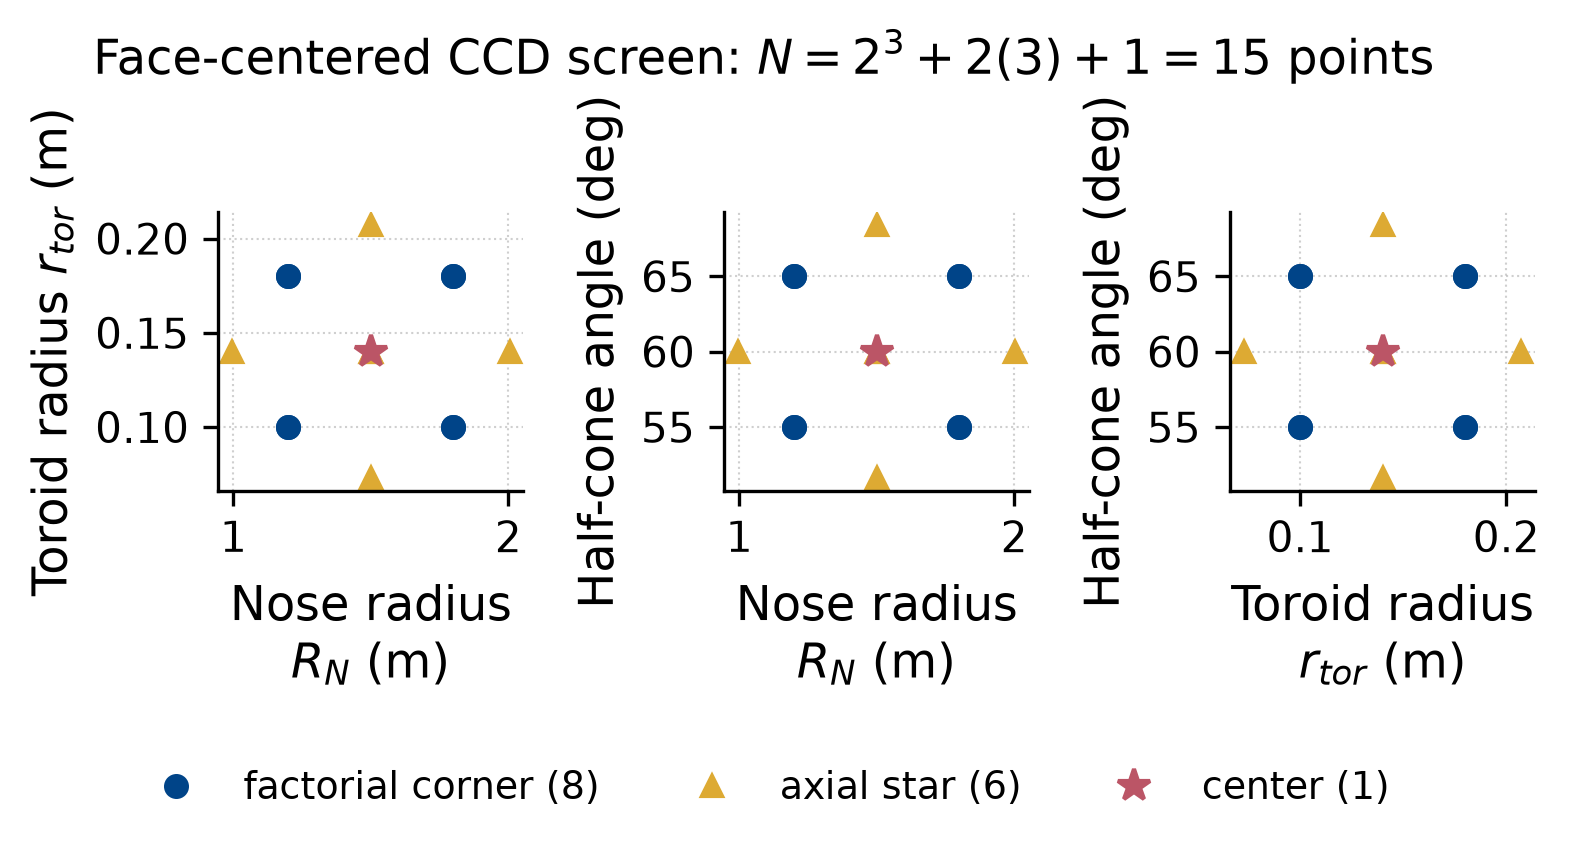
\includegraphics[width=0.9\textwidth,height=0.4\textheight,keepaspectratio]{figures/so_ccd_screen.png}
  \par\vspace{0.5em}
  \small
  \begin{itemize}
    \item \textbf{CCD-15 (screen):} face-centered, 3 vars. Captures curvature + corners. Run first as validated candidate.
    \item \textbf{LHS-20 (base):} space-filling. Feeds Kriging surrogate; fills gaps CCD leaves.
    \item \textbf{BO 50 steps (refine):} EI-driven; spends budget where info gain is highest.
    \item \textbf{Why both:} CCD alone misses space coverage; LHS alone misses curvature. Together: screen + surrogate + refine.
  \end{itemize}
\end{frame}

\PlotFrame{DoE: LHS CUBE SAMPLING}
% Caption trimmed to 2 RENDERED lines (measured with \prevgraf at \small over
% \textwidth = 404.03pt, not guessed from the source line count) so that the
% \MaxTextLines assertion stays honest about the house 1-2 line body budget.
  {\MaxTextLines{2}%
   LHS-20 space-filling base design in the 3-variable cube ($R_N$, $r_{tor}$, $\theta_c$).
   CCD-15 covers corners/edges/centre; LHS-20 fills the rest for Kriging,
   and BO refines within it.}
  {so_lhs_cube}

\PlotFrame{REDEMPTION 3b: DESIGN OF EXPERIMENTS -- THE CCD SCREEN}
  {\MaxTextLines{2}%
   Face-centred 15-point CCD over $k=3$ variables ($R_N$, $r_t$, $\theta_c$):
   $2^3{=}8$ factorial, $2k{=}6$ axial, 1 centre. CCD supplies curvature and
   corner/face coverage; LHS supplies the space-filling base for Kriging.}
  {so_ccd_screen}

% inserted between DoE sampling and the produced geometry grid:
% state the optimization ordering explicitly.
\PlotFrame{REDEMPTION 3c: OPTIMIZATION STAGE}
  {\MaxTextLines{2}%
   CCD gives the validated first candidate; the 20-point LHS base design and
   50 BO improvement steps then optimize it (Bayesian plot follows).}
  {so_bo_convergence}

% moved next to the DoE/CCD slide: 70-evaluation Bayesian design plot.
% Figure copied from CurrentThesisFinalReport/figures/bo_optimization_3d.png
% because it is the readable, titled thesis version; it shows final best 1.6051.
\PlotFrame{OPTIMIZATION DIAGNOSTIC: 70-EVAL BAYESIAN CAMPAIGN}
% Caption trimmed to 2 RENDERED lines (measured with \prevgraf at \small over
% \textwidth = 404.03pt, not guessed from the source line count) so that the
% \MaxTextLines assertion stays honest about the house 1-2 line body budget.
% The Source citation is folded into the body, not deleted: the house rule
% requires every number to name the file it came from.
  {\MaxTextLines{2}%
   BO saturates after ~50 evals (cost 1.6051); later steps add no improvement.
   Search diagnostic, not DSMC validation.
   Source: results/99\_shared/geometry/bo\_optimization\_3d.png.}
  {so_bo_3d}

% produced geometry grid selected from the official run: use the shipped render
% (avoid generated typesetting; image is the source truth).
\PlotFrame{DESIGN-SPACE RESULT: GEOMETRY GRID}
  {\MaxTextLines{2}%
   What this is: sampled geometry candidates, not a DSMC validation result.
   Source: results/99\_shared/geometry/hiad\_geometry\_grid.png.}
  {hiad_geometry_grid}

\section{VALIDATION}
\PlotFrame{TPS RESULT: BACKFACE CHECK}
  {\MaxTextLines{2}%
   What this is: TPS survivability/backface result, not optimization.
   Source: results/00\_reference/plots/derived/survivability\_assessment.png.}
  {so_tps_backface}
\PlotFrame{TPS RESULT: PLY STACK TEMPERATURE}
  {\MaxTextLines{2}%
   What this is: per-ply TPS temperature field from the latest per-ply solve,
   not optimization. Source: results/00\_reference/plots/tps\_per\_ply/
   ply\_stack\_temperature\_heatmap.png.}
  {so_ply_stack_temperature}
\PlotFrame{TPS RESULT: PEAK PLY PROFILE}
  {\MaxTextLines{2}%
   What this is: through-thickness TPS profile at the peak-flux element, not
   optimization. Source: results/00\_reference/plots/tps\_per\_ply/
   ply\_temperature\_profile\_peak\_element.png.}
  {so_tps_ply_profile_peak}
\PlotFrame{VALIDATION RESULT: HYBRID DSMC GATE}
  {\MaxTextLines{2}%
   What this is: cross-mission validation comparison for the optimized
   candidate, not another optimization plot. Source: results/00\_reference/
   plots/validation\_pipeline/multi\_mission\_comparison.png.}
  {so_gate_comparison}
% SOP evidence item 9: Limitations and next step. Always present, never omitted.
% Each limitation cites the frame that carries the claim it limits.
\begin{frame}{LIMITATIONS AND NEXT STEP}
  \footnotesize
  Single-point validation: the 51.8 km / 3378 m/s anchor is the only DSMC
  reference point (REDEMPTION 3a2), so trajectory-wide statements remain PINN
  overview (REDEMPTION 3a3), not validated extents.\\
  Resistance basis: reconciled 2026-10-19. The balance uses the thesis
  schedule $R_{tot}=0.305583$ m$^2$K/W (REDEMPTION 1e), the $\Sigma$(t/k) of
  the 7.131 mm 5-ply stack. The older $0.25605$ belonged to the superseded
  $6.35$ mm flown IRVE-3 stack and is retired (stellarorion\_types.ads:760).\\
  Next step: re-run the surrogate cost on the latest reference values, re-issue
  the DSMC gate, then refresh the per-ply figures in a single commit.
\end{frame}

\section{ANSWER: OPTIMIZATION RESULT}
% Added after the STATUS UPDATE frame at the owner's request: result page using
% the final thesis 2x2 reference-vs-optimized topology and the DSMC-gated result.
% Figure copied from CurrentThesisFinalReport/figures/optimization_comparison.png.
% Numbers: chapter_04_results.tex, tab:bo_before_after, official run 2026-09-26.


\section{CONTEXT}
\PlotFrame{OPTIMIZATION COMPARISON: TOPOLOGY (2x2)}
  {\MaxTextLines{2}%
   Topology comparison of baseline vs. optimized geometry.
   Source: results/99\_shared/geometry/optimization\_comparison.png.}
  {so_optcomp}

\PlotFrame{SURFACE PROFILE CHECK}
  {\MaxTextLines{2}%
   Surface profile check of the optimized geometry.
   Source: results/99\_shared/geometry/surf\_profile\_check.png.}
  {so_surfprofile}

\begin{frame}{RESULT TABLE: BASELINE VS. OPTIMIZED}
  \scriptsize
  \renewcommand{\arraystretch}{1.05}
  \begin{tabular}{@{}lrrr@{}}
    \hline
    \textbf{Parameter} & \textbf{Baseline} & \textbf{Optimized} & \textbf{$\Delta$} \\
    \hline
    \multicolumn{4}{@{}l}{\textbf{Geometry and closed-form surrogate}} \\
    Nose radius $R_N$ & 1.5000 m & 2.9714 m & $+98.10\%$ \\
    Torus radius $r_{tor}$ & 0.1350 m & 0.0885 m & $-34.47\%$ \\
    Half-cone angle $\theta_c$ & $60.00^\circ$ & $40.15^\circ$ & $-33.09\%$ \\
    Drag coefficient $C_d$ & 1.6073 & 1.5597 & $-2.96\%$ \\
    Sutton--Graves heat flux & 15.36 W/cm$^2$ & 11.47 W/cm$^2$ & $-28.95\%$ \\
    Total heat load $Q(\mathbf{x})$ & 219.10 J/cm$^2$ & 155.67 J/cm$^2$ & $-28.95\%$ \\
    Cost $J(\mathbf{x})$ & 2.1626 & 1.6051 & $-25.78\%$ \\
    \hline
    \multicolumn{4}{@{}l}{\textbf{DSMC (baseline run / latest gate re-simulation)}} \\
    Drag coefficient $C_d$ & 1.7655 & 2.5294 & $+43.3\%$ \\
    Total heat load $Q$ & 165.72 J/cm$^2$ & 77.93 J/cm$^2$ & $-53.0\%$ \\
    Peak deceleration & 16.55 g & 14.01 g & $-15.3\%$ \\
    Ballistic coefficient $\beta$ & 27.70 kg/m$^2$ & 10.06 kg/m$^2$ & $-63.7\%$ \\
    Lift coefficient $C_l$ & $-0.5268$ & $-1.0767$ & $+104.4\%$ \\
    \hline
  \end{tabular}
  \par{\scriptsize Source: Latest attempt; superseded run deleted 2026-10-14 (latest attempt retained).}
\end{frame}

% =====================================================================
% NARRATION REVAMP: PLACEHOLDER SCAFFOLD
% ---------------------------------------------------------------------
% Added 2026-10-21 on the owner's directive. The target narration order
% is written out in full in the NARRATION REVAMP comment block at the
% top of this file.
%
% These frames carry NO content. Each one is a marker naming the block
% it stands for, so the deck holds the narration skeleton before any
% prose is written. The comment above each frame states the position
% that frame must occupy in the final deck; once a frame is filled it
% moves to that position as a cut-and-paste of one
% \begin{frame}...\end{frame} block.
%
% House rules that still bind these frames: at most two lines of body
% text, no bullet lists, no U+2014, every number cites its source file,
% and frametitles stay short enough for the fixed-width frametitle band.
% =====================================================================
\section{NARRATION REVAMP: PLACEHOLDER SCAFFOLD}

% [ Intro start ]
% Target position: the opening of the deck, ahead of the OUTLINE frame.
\begin{frame}{PLACEHOLDER 0: TITLE (INTRO)}
  \small\textit{Intro block 0: title. Frame exists; narration pending.}
\end{frame}
% [ intro end ]

% [ recall start ]
% Target position: immediately after the OUTLINE frame.
\begin{frame}{PLACEHOLDER 1: LATAR BELAKANG OVERVIEW}
  \small\textit{Recall block 1: background overview. Narration pending.}
\end{frame}

% Target position: immediately after PLACEHOLDER 1.
\begin{frame}{PLACEHOLDER 2: TUJUAN AND RESEARCH SCOPE}
  \small\textit{Recall block 2: objective and scope limit. Narration pending.}
\end{frame}

% Target position: immediately after PLACEHOLDER 2.
\begin{frame}{PLACEHOLDER 3: METHODOLOGY AND REASONING}
  \small\textit{Recall block 3: methodology and its reasoning. Narration pending.}
\end{frame}

% Target position: around the existing PREVIOUS PROBLEM frame, which
% already lists the three prior issues; this frame is the narration that
% frames them.
\begin{frame}{PLACEHOLDER 4: PREVIOUS ISSUES}
  \small\textit{Recall block 4: previous issues. Narration pending.}
\end{frame}
% [ recall end ]

% [ Current progress start ]
% Target position: around the existing STATUS UPDATE frame, which
% already carries the work-item percentages; this frame is the overall
% progress narration and deliberately excludes the resolution detail.
\begin{frame}{PLACEHOLDER 5: OVERALL PROGRESS}
  \small\textit{Current progress block 5: overall progress. Narration pending.}
\end{frame}
% [ Current progress end ]

% Target position: after the field-evidence and optimization blocks.
\begin{frame}{PLACEHOLDER 6: ISSUE, RESOLUTION, UPDATE}
  \small\textit{Current progress block 6: issue, attempt, update. Narration pending.}
\end{frame}

% The two required plots. The owner's note asks for the CFD case and the
% optimized case to be stated in writing as well as plotted, so each
% frame holds the reserved space plus the note on what the plot must
% show. Neither uses \PlotFrame: no image exists yet, and the missing
% image diagnostic would put a forbidden pattern into the built PDF.

% [ Ending start ]
% Target position: the last content frame of the deck.
\begin{frame}{PLACEHOLDER 7: CONCLUSION}
  \small\textit{Ending block: conclusion. Narration pending.}
\end{frame}
% [ Ending end ]

\end{document}
